\chapter{Spektroskopi Inframerah}\label{ch:g11:infrared}

Di rak laboratorium berdiri sebotol cairan tak berwarna yang labelnya
telah sobek. Isinya mungkin \omterm{def:g11:functional-groups:alcohol}{alkohol}, \omterm{def:g11:functional-groups:carbonyl}{keton}, atau asam: tiga keluarga
yang tampak persis sama di dalam botol. Setetes cairan itu diletakkan di
atas kristal spektrometer inframerah, dua menit menunggu, dan sebuah
grafik muncul di layar yang menjawab pertanyaan itu. Ikatan-ikatan dalam
sebuah \omterm{def:g7:atoms-and-molecules:molecule}{molekul} bergetar, dan setiap jenis ikatan menyerap cahaya
inframerah dengan frekuensinya sendiri: \omterm{def:g11:infrared:spectrum}{spektrum inframerah} adalah
daftar ikatan yang ada.

\begin{recall}
\omterm{def:g11:functional-groups:functional-group}{Gugus fungsi} dan keluarga senyawa (\cref{ch:g11:functional-groups}).
\omterm{def:g11:absorbance:spectrum}{Spektrum serapan} memperlihatkan berapa banyak cahaya yang diserap sebuah
zat pada setiap panjang gelombang (\cref{ch:g11:absorbance}). \omterm{def:g11:polarity-and-cohesion:hydrogen-bond}{Ikatan
hidrogen} menghubungkan gugus \ce{O-H} dengan \omterm{def:g7:atoms-and-molecules:molecule}{molekul-molekul} tetangganya
(\cref{ch:g11:polarity-and-cohesion}).
\end{recall}

\section{Ikatan bergetar}

\omterm{def:g10:lewis-and-shape:covalent-bond}{Ikatan kovalen} tidak kaku: kedua \omterm{def:g7:atoms-and-molecules:atom}{atomnya} bergetar, saling mendekat dan
menjauh jutaan juta kali per detik, seperti dua bola yang dihubungkan
oleh pegas. Pegas yang lebih kaku (\omterm{def:g10:lewis-and-shape:multiple-bond}{ikatan rangkap dua} alih-alih ikatan
tunggal) atau bola yang lebih ringan (\omterm{def:g7:atoms-and-molecules:atom}{atom} hidrogen alih-alih \omterm{def:g7:atoms-and-molecules:atom}{atom}
karbon) bergetar lebih cepat. Sebuah ikatan dapat menyerap cahaya
inframerah yang frekuensinya sesuai dengan getarannya sendiri: cahaya
inframerah, yang tidak terlihat oleh mata, memiliki panjang gelombang
beberapa mikrometer sampai beberapa puluh mikrometer.

\begin{omfigure}
\begin{tikzpicture}[font=\small]
  \node[aC] (c) at (0,0) {};
  \node[aO] (o) at (2.2,0) {};
  \draw[decorate, decoration={coil, aspect=0.4, segment length=4pt,
    amplitude=4pt}, thick, black!60] (c.east) -- (o.west);
  \draw[<->, omProp, thick] (-0.9,0) -- (-0.45,0);
  \draw[<->, omProp, thick] (2.65,0) -- (3.1,0);
  \node[anchor=north] at (1.1,-0.5) {ikatan yang memanjang dan memendek};
  \node[aO] (o1) at (5.3,0) {};
  \node[aH] (h1) at (6.7,0) {};
  \draw[decorate, decoration={coil, aspect=0.4, segment length=3pt,
    amplitude=3pt}, thick, black!60] (o1.east) -- (h1.west);
  \draw[<->, omProp, thick] (7.0,0) -- (7.7,0);
  \node[anchor=north, align=center] at (6.2,-0.5) {atom hidrogen yang ringan:\\ getaran lebih cepat};
\end{tikzpicture}

{\small Ikatan yang digambarkan sebagai pegas di antara dua bola.
Getarannya memiliki frekuensi yang ditentukan oleh kekakuan ikatan dan
massa \omterm{def:g7:atoms-and-molecules:atom}{atom-atomnya}; cahaya inframerah dengan frekuensi itu diserap.}
\end{omfigure}

\begin{definition}[Bilangan gelombang]\label{def:g11:infrared:wavenumber}
Yang disebut \emph{bilangan gelombang}\index{bilangan gelombang}
$\sigma$ sebuah cahaya adalah kebalikan panjang gelombangnya,
$\sigma = 1/\lambda$. Dalam spektroskopi inframerah, bilangan gelombang
dinyatakan dalam \si{cm^{-1}}: banyaknya panjang gelombang dalam satu
sentimeter. Bilangan gelombang yang lebih besar berarti panjang
gelombang yang lebih pendek dan getaran yang lebih cepat.
\end{definition}

\begin{example}[Dari bilangan gelombang ke panjang gelombang]\label{ex:g11:infrared:convert}
Pita pada $\sigma = \qty{2000}{cm^{-1}}$ sesuai dengan
$\lambda = 1/2000 = \qty{5.0e-4}{cm} = \qty{5.0}{\micro m}$. \omterm{def:g11:infrared:spectrum}{Spektrum
inframerah} biasanya terbentang dari \qty{4000}{cm^{-1}}
(\qty{2.5}{\micro m}) sampai \qty{500}{cm^{-1}} (\qty{20}{\micro m}).
\end{example}

\section{Membaca spektrum inframerah}

\begin{definition}[Spektrum inframerah, transmitans]\label{def:g11:infrared:spectrum}
Yang disebut \emph{transmitans}\index{transmitans} $T$ sebuah sampel
pada \omterm{def:g11:infrared:wavenumber}{bilangan gelombang} tertentu adalah persentase cahaya inframerah
yang menembusnya: \qty{100}{\percent} jika tidak ada yang diserap. Yang
disebut \emph{spektrum inframerah}\index{spektrum inframerah} sebuah
senyawa adalah grafik $T$ terhadap \omterm{def:g11:infrared:wavenumber}{bilangan gelombang}, yang menurut
kesepakatan digambar dengan \omterm{def:g11:infrared:wavenumber}{bilangan gelombang} yang mengecil dari kiri
ke kanan.
\end{definition}

\begin{definition}[Pita serapan, daerah sidik jari]\label{def:g11:infrared:band}
Yang disebut \emph{pita serapan}\index{pita serapan} adalah lekukan ke
bawah pada \omterm{def:g11:infrared:spectrum}{transmitans}: cahaya dengan bilangan-bilangan gelombang itu
diserap oleh sebuah ikatan. Letaknya menunjukkan ikatan yang mana, lebar
dan dalamnya melengkapi gambarannya. Di bawah sekitar
\qty{1500}{cm^{-1}}, spektrum dipenuhi pita-pita yang bergantung pada
seluruh \omterm{def:g7:atoms-and-molecules:molecule}{molekul}: \emph{daerah sidik jari}\index{daerah sidik jari} ini
mengenali sebuah senyawa dengan membandingkannya dengan spektrum yang
sudah diketahui, tetapi sukar dibaca ikatan demi ikatan.
\end{definition}

\begin{inthelab}[Merekam spektrum]
Kebanyakan spektrometer di sekolah dan universitas kini memakai kristal
intan kecil: setetes cairan, atau beberapa butir padatan yang ditekan
oleh penjepit, diletakkan di atas kristal, dan berkas inframerah yang
menyerempet permukaannya memeriksa sampel itu. Kristal itu mula-mula
direkam dalam keadaan bersih (``latar belakang''), yang berperan sebagai
blanko. Kristal dibersihkan dengan tisu dan sedikit \omterm{def:g6:solutions-and-solubility:solute}{pelarut} di antara
dua sampel.
\end{inthelab}

\section{Pita-pita khas}

\begin{proposition}[Setiap jenis ikatan memiliki pitanya]\label{prop:g11:infrared:bands}
% ledger: ir:OH-free, ir:OH-bonded, ir:OH-acid, ir:NH, ir:CH, ir:CO-aldehyde, ir:CO-ketone, ir:CO-ester, ir:CO-acid, ir:CC-double, ir:CO-single
Setiap jenis ikatan menyerap pada rentang \omterm{def:g11:infrared:wavenumber}{bilangan gelombang} yang khas,
hampir sama dari satu \omterm{def:g7:atoms-and-molecules:molecule}{molekul} ke \omterm{def:g7:atoms-and-molecules:molecule}{molekul} lain:
\begin{center}
\small
\begin{tabular}{lll}
\hline
ikatan & \omterm{def:g11:infrared:wavenumber}{bilangan gelombang} (\si{cm^{-1}}) & tampilan \\
\hline
\ce{O-H} bebas (gas, encer) & sekitar 3600 & tajam \\
\ce{O-H} terikat hidrogen (\omterm{def:g11:functional-groups:alcohol}{alkohol} cair) & 3300--3400 & lebar, kuat \\
\ce{O-H} \omterm{def:g11:functional-groups:carboxylic-acid}{asam karboksilat} & 2500--3300 & sangat lebar \\
\ce{N-H} \omterm{def:g11:functional-groups:amine}{amina} & 3300--3500 & sedang (dua pita untuk \ce{-NH2}) \\
\ce{C-H} rantai & 2850--2960 & kuat \\
\ce{C=O} \omterm{def:g11:functional-groups:carboxylic-acid}{ester} & sekitar 1735 & sangat kuat, tajam \\
\ce{C=O} \omterm{def:g11:functional-groups:carbonyl}{aldehida} & sekitar 1730 & sangat kuat, tajam \\
\ce{C=O} \omterm{def:g11:functional-groups:carbonyl}{keton} & sekitar 1715 & sangat kuat, tajam \\
\ce{C=O} \omterm{def:g11:functional-groups:carboxylic-acid}{asam karboksilat} & sekitar 1710 & sangat kuat, lebih lebar \\
\ce{C=C} & sekitar 1650 & sedang \\
\ce{C-O} \omterm{def:g11:functional-groups:alcohol}{alkohol} & sekitar 1050 & kuat \\
\hline
\end{tabular}
\end{center}
\end{proposition}

\begin{proof}
Rentang-rentang ini diukur pada banyak senyawa. Rentang itu
berkelompok menurut ikatan karena getaran sebuah ikatan terutama
bergantung pada ikatan itu sendiri dan kedua \omterm{def:g7:atoms-and-molecules:atom}{atomnya}, dan hanya sedikit
pada bagian \omterm{def:g7:atoms-and-molecules:molecule}{molekul} yang lain.
\end{proof}

\begin{omfigure}
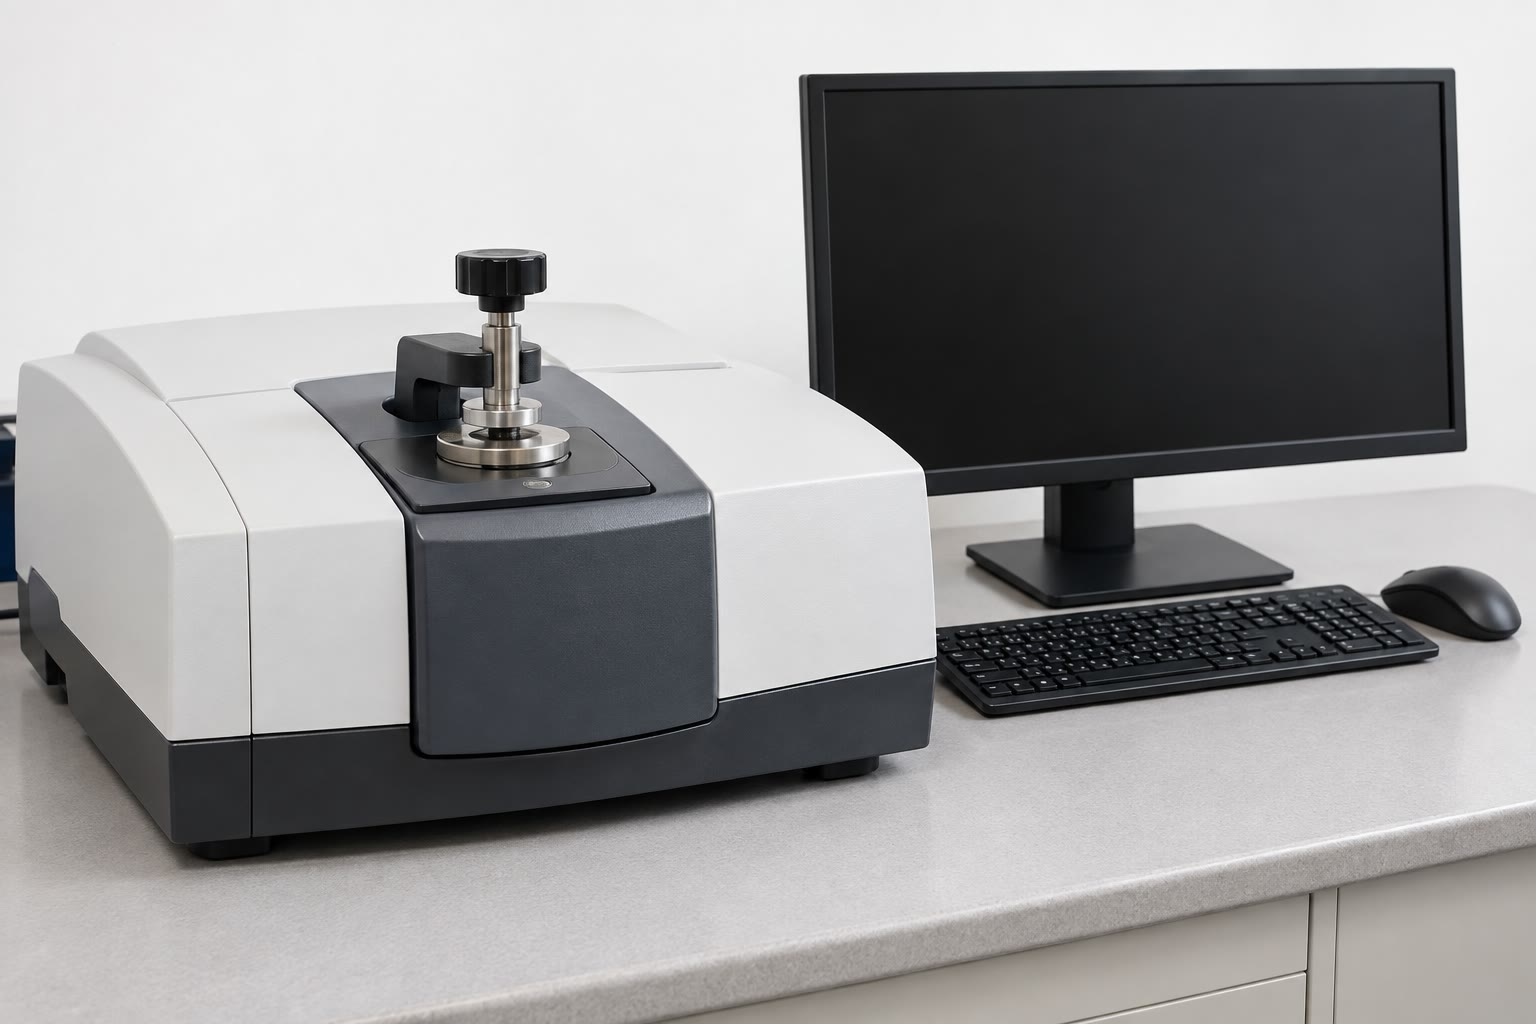
\includegraphics[width=0.48\linewidth]{images/book1/ai/g11-ftir.jpg}

{\small Spektrometer inframerah meja dengan kristal dan penjepitnya.}
\end{omfigure}

\begin{omfigure}
\begin{tikzpicture}[font=\small, x=0.0036cm, y=0.5cm]
  % wavenumber axis reversed: x = 4000 - sigma
  \fill[black!8] (2500,0.2) rectangle (3500,7.6);
  \node[font=\footnotesize, align=center, black!60] at (3000,6.8) {daerah\\ sidik jari};
  \draw[->] (0,0) -- (3600,0) node[right] {$\sigma$};
  \foreach \s in {4000,3500,3000,2500,2000,1500,1000,500}
    \draw ({4000-\s},0) -- ({4000-\s},-0.15) node[below, font=\footnotesize] {\s};
  \node[below=12pt] at (1800,-0.3) {bilangan gelombang (\si{cm^{-1}})};
  \foreach \a/\b/\y/\c/\l in {
      3600/3600/7/omDef/{\ce{O-H} bebas},
      3300/3400/6/omDef/{\ce{O-H} berikatan H},
      2500/3300/5/omThm/{\ce{O-H} asam},
      3300/3500/4/omMeth/{\ce{N-H}},
      2850/2960/3/black!60/{\ce{C-H}},
      1700/1740/2/omProp/{\ce{C=O}},
      1050/1050/1/black!45/{\ce{C-O}}} {
    \fill[\c, rounded corners=1pt] ({4000-\b-12},{\y-0.25}) rectangle ({4000-\a+12},{\y+0.25});
    \node[anchor=west, font=\footnotesize] at ({4000-\a+40},\y) {\l};
  }
\end{tikzpicture}

{\small Tempat ikatan-ikatan utama menyerap. Pita \ce{O-H} dan \ce{N-H}
berada di kiri, pita \ce{C=O}, biasanya yang paling kuat, di sekitar
\qty{1700}{cm^{-1}}; di bawah \qty{1500}{cm^{-1}} terbentang \omterm{def:g11:infrared:band}{daerah
sidik jari}.}
\end{omfigure}

\begin{proposition}[Ikatan hidrogen melebarkan pita O--H]\label{prop:g11:infrared:hbond}
% ledger: ir:OH-free, ir:OH-bonded, ir:ethanol-OH
Jika gugus-gugus \ce{O-H} dihubungkan oleh \omterm{def:g11:polarity-and-cohesion:hydrogen-bond}{ikatan hidrogen}, seperti pada
\omterm{def:g11:functional-groups:alcohol}{alkohol} cair, pitanya lebar dan terletak pada \omterm{def:g11:infrared:wavenumber}{bilangan gelombang} yang
lebih rendah (sekitar 3300--\qty{3400}{cm^{-1}}); tanpa \omterm{def:g11:polarity-and-cohesion:hydrogen-bond}{ikatan hidrogen},
seperti dalam keadaan gas, pitanya tajam dan berada di sekitar
\qty{3600}{cm^{-1}}.
\end{proposition}

\begin{proof}
Diterima tanpa bukti: \omterm{def:g11:polarity-and-cohesion:hydrogen-bond}{ikatan hidrogen} menarik \omterm{def:g7:atoms-and-molecules:atom}{atom} hidrogen dan
melonggarkan ikatan \ce{O-H}, yang lalu bergetar lebih lambat; dan karena
setiap \omterm{def:g7:atoms-and-molecules:molecule}{molekul} terikat sedikit berbeda, pitanya menyebar dalam suatu
rentang.
\end{proof}

\section{Mengenali gugus fungsi}


\begin{method}[Membaca spektrum inframerah]\label{met:g11:infrared:reading}
\begin{enumerate}
  \item Lihatlah dulu bagian di atas \qty{1500}{cm^{-1}}; biarkan \omterm{def:g11:infrared:band}{daerah
        sidik jari} untuk dibandingkan dengan spektrum yang sudah dikenal.
  \item Di sekitar \qty{1700}{cm^{-1}}: pita yang sangat kuat berarti
        gugus \ce{C=O} (\omterm{def:g11:functional-groups:carbonyl}{aldehida}, \omterm{def:g11:functional-groups:carbonyl}{keton}, asam, \omterm{def:g11:functional-groups:carboxylic-acid}{ester}, \omterm{def:g11:functional-groups:amine}{amida}).
  \item Antara 2500 dan \qty{3700}{cm^{-1}}: pita lebar di sekitar
        \qty{3350}{cm^{-1}} berarti \ce{O-H} \omterm{def:g11:functional-groups:alcohol}{alkohol}; pita yang sangat
        lebar dari 2500 sampai \qty{3300}{cm^{-1}} disertai \ce{C=O}
        berarti \omterm{def:g11:functional-groups:carboxylic-acid}{asam karboksilat}; pita-pita sedang pada
        3300--\qty{3500}{cm^{-1}} berarti \ce{N-H}.
  \item Gabungkan dengan \omterm{def:g11:organic-skeletons:formulas}{rumus molekulnya} untuk memilih keluarganya, lalu
        periksalah dengan letak pita \ce{C=O} jika ada.
\end{enumerate}
\end{method}

\begin{omfigure}
\newcommand{\irpanel}[2]{%
\begin{tikzpicture}
\begin{axis}[width=0.96\linewidth, height=3.9cm, x dir=reverse, xmin=500,
    xmax=4000, ymin=0, ymax=105, xtick={4000,3000,2000,1000},
    /pgf/number format/1000 sep={},
    ytick={0,50,100}, tick label style={font=\scriptsize},
    label style={font=\scriptsize}, ylabel={$T$ (\%)}, axis lines*=left,
    title={\small #2}, title style={yshift=-4pt}]
  \addplot[thick, omDef] table[x=sigma, y=#1] {figdata/out/grade-11-infrared.dat};
\end{axis}
\end{tikzpicture}}
\begin{minipage}{0.49\linewidth}\irpanel{ethanolL}{A: etanol (cair)}\end{minipage}\hfill
\begin{minipage}{0.49\linewidth}\irpanel{ethanolG}{B: etanol (gas)}\end{minipage}

\begin{minipage}{0.49\linewidth}\irpanel{propanone}{C: propanon}\end{minipage}\hfill
\begin{minipage}{0.49\linewidth}\irpanel{acid}{D: asam etanoat}\end{minipage}

\begin{minipage}{0.49\linewidth}\irpanel{ester}{E: etil etanoat}\end{minipage}\hfill
\begin{minipage}{0.49\linewidth}\irpanel{amine}{F: etanamina}\end{minipage}

{\small \omterm{def:g11:infrared:spectrum}{Spektrum inframerah} enam senyawa, \omterm{def:g11:infrared:wavenumber}{bilangan gelombang} dalam
\si{cm^{-1}} (mengecil ke kanan). Hanya pita-pita yang dibahas dalam bab
ini yang digambar; letaknya berasal dari spektrum terukur dan tabel,
bentuknya dari sebuah model sederhana.}
\end{omfigure}

\begin{example}[Membaca keenam spektrum]\label{ex:g11:infrared:six}
% ledger: ir:OH-bonded, ir:ethanol-OH, ir:CO-ketone, ir:OH-acid, ir:CO-acid, ir:CO-ester, ir:ethylethanoate-COC, ir:NH
Etanol (A) memperlihatkan pita \ce{O-H} yang lebar di sekitar
\qty{3350}{cm^{-1}}, pita-pita \ce{C-H} tepat di bawah
\qty{3000}{cm^{-1}}, dan pita \ce{C-O} yang kuat di sekitar
\qty{1050}{cm^{-1}}, tetapi tidak ada apa-apa di sekitar
\qty{1700}{cm^{-1}}. Dalam keadaan gas (B), pita \ce{O-H}-nya menjadi
garis tajam pada \qty{3666}{cm^{-1}}. Propanon (C) tidak memiliki pita
\ce{O-H} tetapi memiliki \ce{C=O} yang sangat kuat pada
\qty{1715}{cm^{-1}}. Asam etanoat (D) memperlihatkan keduanya: pita
\ce{O-H} yang sangat lebar dari 2500 sampai \qty{3300}{cm^{-1}} dan
\ce{C=O} pada \qty{1710}{cm^{-1}}. Etil etanoat (E) memiliki \ce{C=O}
pada \qty{1735}{cm^{-1}} dan \ce{C-O} yang kuat di sekitar
\qty{1240}{cm^{-1}}, dan tidak ada \ce{O-H}. Etanamina (F) memperlihatkan
dua pita \ce{N-H} sedang di atas \qty{3300}{cm^{-1}}.
\end{example}

\section{Latihan}

\begin{exercise}[$\star$]\label{exo:g11:infrared:1}
Ubahlah menjadi panjang gelombang dalam mikrometer:
$\sigma = \qty{3300}{cm^{-1}}$ dan $\sigma = \qty{1050}{cm^{-1}}$.
Manakah yang sesuai dengan getaran yang lebih cepat?
\end{exercise}

\begin{exercise}[$\star$]\label{exo:g11:infrared:2}
Panjang gelombang \qty{10}{\micro m} diserap. Berikan \omterm{def:g11:infrared:wavenumber}{bilangan
gelombangnya} dalam \si{cm^{-1}}.
\end{exercise}

\begin{exercise}[$\star$]\label{exo:g11:infrared:3}
Ikatan apa yang menyerap: di sekitar \qty{1715}{cm^{-1}}; di sekitar
\qty{3350}{cm^{-1}} (lebar); antara 2850 dan \qty{2960}{cm^{-1}}?
\end{exercise}

\begin{exercise}[$\star$]\label{exo:g11:infrared:4}
Pada spektrum C (propanon), carilah pita yang paling kuat. Pita itu
milik ikatan apa?
\end{exercise}

\begin{exercise}[$\star$]\label{exo:g11:infrared:5}
Mengapa \omterm{def:g11:infrared:spectrum}{spektrum inframerah} digambar dengan sumbu \omterm{def:g11:infrared:spectrum}{transmitans}, dengan
pita-pita yang mengarah ke bawah? Apa arti $T = \qty{100}{\percent}$?
\end{exercise}

\begin{exercise}[$\star\star$]\label{exo:g11:infrared:6}
Sebuah senyawa \ce{C4H8O} memperlihatkan pita yang sangat kuat pada
\qty{1715}{cm^{-1}} dan tidak ada pita di atas \qty{3000}{cm^{-1}}.
Senyawa lain, \ce{C4H10O}, memperlihatkan pita lebar di sekitar
\qty{3350}{cm^{-1}} dan tidak ada pita di sekitar \qty{1700}{cm^{-1}}.
Termasuk keluarga apa keduanya? Usulkan nama untuk masing-masing.
\end{exercise}

\begin{exercise}[$\star\star$]\label{exo:g11:infrared:7}
Jelaskan mengapa pita \ce{O-H} asam etanoat begitu lebar, bahkan lebih
lebar daripada pita etanol cair.
\end{exercise}

\begin{exercise}[$\star\star$]\label{exo:g11:infrared:8}
Bandingkan spektrum A dan B etanol. Apa yang berubah, dan mengapa?
\end{exercise}

\begin{exercise}[$\star\star$]\label{exo:g11:infrared:9}
Propanal dan propanon sama-sama \ce{C3H6O}. Keduanya memperlihatkan pita
\ce{C=O} yang kuat. Dapatkah inframerah membedakan keduanya dari pita
itu saja? Apa lagi yang dapat membantu?
\end{exercise}

\begin{exercise}[$\star\star$]\label{exo:g11:infrared:10}
Sebuah senyawa memperlihatkan pita yang kuat pada \qty{1735}{cm^{-1}},
pita yang kuat di sekitar \qty{1240}{cm^{-1}}, dan tidak ada apa-apa di
atas \qty{3000}{cm^{-1}}. Rumusnya \ce{C4H8O2}. Keluarga apa? Apakah
asam etanoat mungkin? Asam butanoat?
\end{exercise}

\begin{exercise}[$\star\star$]\label{exo:g11:infrared:11}
Spektrum mana dari keenam spektrum itu yang paling mirip dengan
spektrum \omterm{def:g7:atoms-and-molecules:molecule}{molekul} propan-1-ol? Asam propanoat? Jelaskan.
\end{exercise}

\begin{exercise}[$\star\star\star$]\label{exo:g11:infrared:12}
Propan-2-ol dapat dioksidasi menjadi propanon. Seorang siswa mengikuti
reaksi itu dengan merekam spektrum sampel yang diambil setiap sepuluh
menit. Uraikan bagaimana spektrum-spektrum itu berubah. Bagaimana ia
mengetahui bahwa reaksinya telah selesai?
\end{exercise}

\begin{exercise}[$\star\star\star$]\label{exo:g11:infrared:13}
Asam butanoat dan etil etanoat adalah \omterm{def:g11:organic-skeletons:isomer}{isomer}, \ce{C4H8O2}. Uraikan dua
perbedaan antara \omterm{def:g11:infrared:spectrum}{spektrum inframerah} keduanya, dan jelaskan.
\end{exercise}

\begin{exercise}[$\star\star\star$]\label{exo:g11:infrared:14}
Sebuah sampel etil etanoat memperlihatkan, selain pita-pita yang
diharapkan, pita lebar yang lemah di sekitar \qty{3350}{cm^{-1}}.
Usulkan dua pengotor yang dapat menyebabkannya (pikirkan cara \omterm{def:g11:functional-groups:carboxylic-acid}{ester}
dibuat, dan \omterm{def:g4:air-a-mixture-of-gases:air}{udara}). Bagaimana sampel itu dapat diperiksa?
\end{exercise}

\begin{exercise}[$\star\star\star$]\label{exo:g11:infrared:15}
Pita \ce{C=O} \omterm{def:g11:functional-groups:carbonyl}{keton} terletak di sekitar \qty{1715}{cm^{-1}}, pita
\ce{C=C} di sekitar \qty{1650}{cm^{-1}}, dan pita \ce{C-O} di sekitar
\qty{1050}{cm^{-1}}. Dengan gambaran dua bola pada sebuah pegas,
jelaskan mengapa \omterm{def:g10:lewis-and-shape:multiple-bond}{ikatan rangkap dua} \ce{C=O} bergetar lebih cepat
daripada ikatan tunggal \ce{C-O}. Mengapa pita \ce{O-H}, \ce{N-H}, dan
\ce{C-H} semuanya berada pada \omterm{def:g11:infrared:wavenumber}{bilangan gelombang} yang tinggi?
\end{exercise}

\section{Soal: Tiga Botol Tanpa Label}

\begin{problem}[{Soal akhir pekan --- tiga botol kehilangan labelnya: botol
mana berisi apa, dan panjang gelombang berapa yang paling kuat diserap
keton?}]
\label{pb:g11:infrared:1}
% ledger: ir:OH-bonded, ir:OH-acid, ir:CO-ketone, ir:CO-acid, ir:CO-single
Tiga botol berisi cairan tak berwarna kehilangan labelnya. Daftar
persediaan menyebutkan bahwa isinya etanol, propanon, dan asam etanoat.
Spektrumnya direkam: botol 1 memberikan spektrum seperti A, botol 2
seperti D, botol 3 seperti C.

\medskip
\noindent\textbf{Bagian I --- Calon-calonnya.}
\begin{enumerate}
  \item Tuliskan \omterm{def:g11:organic-skeletons:formulas}{rumus struktur ringkas} etanol, propanon, dan asam
        etanoat.
  \item Berikan \omterm{def:g11:organic-skeletons:formulas}{rumus molekulnya}.
  \item Sebutkan \omterm{def:g11:functional-groups:functional-group}{gugus fungsi} masing-masing.
  \item Ikatan mana pada masing-masing yang seharusnya memberikan pita di
        atas \qty{1500}{cm^{-1}}?
\end{enumerate}

\medskip
\noindent\textbf{Bagian II --- Spektrum-spektrumnya.}
\begin{enumerate}[resume]
  \item Botol 1: adakah pita \ce{C=O}? Pita \ce{O-H}? Senyawa apakah
        itu?
  \item Botol 2: uraikan dua cirinya yang paling menonjol. Senyawa apa?
  \item Botol 3: senyawa apa? Pita mana yang menentukan?
  \item Dapatkah baunya membedakan ketiganya? Mengapa lebih baik tidak
        mencobanya?
  \item Mengapa pita \ce{O-H} botol 2 lebih lebar daripada pita botol 1?
\end{enumerate}

\medskip
\noindent\textbf{Bagian III --- \omterm{def:g11:organic-skeletons:isomer}{Isomer}.}
\begin{enumerate}[resume]
  \item Metoksimetana adalah \omterm{def:g11:organic-skeletons:isomer}{isomer} etanol. Tuliskan rumusnya. Pita
        etanol mana yang tidak akan ada pada spektrumnya?
  \item Propanal adalah \omterm{def:g11:organic-skeletons:isomer}{isomer} propanon. Pita mana yang dimiliki
        keduanya? Di mana letaknya pada masing-masing?
  \item Metil metanoat, \ce{HCOO-CH3}, adalah \omterm{def:g11:organic-skeletons:isomer}{isomer} asam etanoat. Pita
        asam mana yang tidak akan ada? Di mana pita \ce{C=O}-nya akan
        terletak?
  \item Mengapa \omterm{def:g11:organic-skeletons:formulas}{rumus molekul} saja tidak dapat mengenali sebuah senyawa,
        sedangkan rumus dan spektrum bersama-sama biasanya dapat?
\end{enumerate}

\medskip
\noindent\textbf{Bagian IV --- Panjang gelombangnya.}
\begin{enumerate}[resume]
  \item Berapa \omterm{def:g11:infrared:wavenumber}{bilangan gelombang} pita propanon yang paling kuat?
  \item Nyatakan dalam \si{m^{-1}}.
  \item Hitung panjang gelombang yang diserap, dalam meter, lalu dalam
        mikrometer.
  \item Apakah cahaya itu terlihat? Termasuk radiasi jenis apa?
  \item Lakukan hal yang sama untuk pita \ce{C-O} etanol di sekitar
        \qty{1050}{cm^{-1}}.
  \item Manakah di antara kedua ikatan itu yang bergetar lebih cepat?
  \item Nyatakan jawaban akhirnya: panjang gelombang berapa yang paling
        kuat diserap ikatan \ce{C=O} pada propanon?
\end{enumerate}
\end{problem}
